\documentclass[a4paper]{article}

%% Language and font encodings
\usepackage[english]{babel}
\usepackage[utf8x]{inputenc}
\usepackage[T1]{fontenc}

%% Sets page size and margins
\usepackage[a4paper,top=3cm,bottom=2cm,left=3cm,right=3cm,marginparwidth=1.75cm]{geometry}

%% Useful packages
\usepackage{amsmath}
\usepackage{graphicx}
\usepackage{pdfpages}
\usepackage{pgfgantt}
\usepackage[colorinlistoftodos]{todonotes}
\usepackage[colorlinks=true, allcolors=blue]{hyperref}
\usepackage{import}

%% Setup syntax highlighting styles
\usepackage{listings}
\usepackage{color}
 
\definecolor{codegreen}{rgb}{0,0.6,0}
\definecolor{codegray}{rgb}{0.5,0.5,0.5}
\definecolor{codepurple}{rgb}{0.58,0,0.82}
\definecolor{backcolor}{rgb}{0.95,0.95,0.92}
 
\lstdefinestyle{mystyle}{
    backgroundcolor=\color{backcolor},   
    commentstyle=\color{codegreen},
    keywordstyle=\color{magenta},
    numberstyle=\tiny\color{codegray},
    stringstyle=\color{codepurple},
    basicstyle=\footnotesize,
    breakatwhitespace=false,         
    breaklines=true,                 
    captionpos=b,                    
    keepspaces=true,                 
    numbers=left,                    
    numbersep=5pt,                  
    showspaces=false,                
    showstringspaces=false,
    showtabs=false,                  
    tabsize=2
}
\lstset{style=mystyle}

\title{Final Report}
\author{Brandon Lee, Rutger Farry, Michael Lee}

\begin{document}

\maketitle

\begin{abstract}
\noindent
The following report evaluates and recaps the purposes and project goals. The following will evaluate project progress, milestones, challenges, problems, proposed solutions, design, and remaining work. The following document will describe these aspects in the technical implementation level as well as in an overall higher level for clarity.
\end{abstract}

\newpage

\tableofcontents

\newpage

% 1
\section{Introduction}
\import{tex/}{introduction}

% 2
\section{Original Requirements Document}

\includepdf[pages={1-},scale=1.0]{pdf/requirements-doc}

% 3
\section{Project Changes – Requirements Document}
\import{tex/}{requirements-doc-changes}

% 4
\section{Original Design Document}
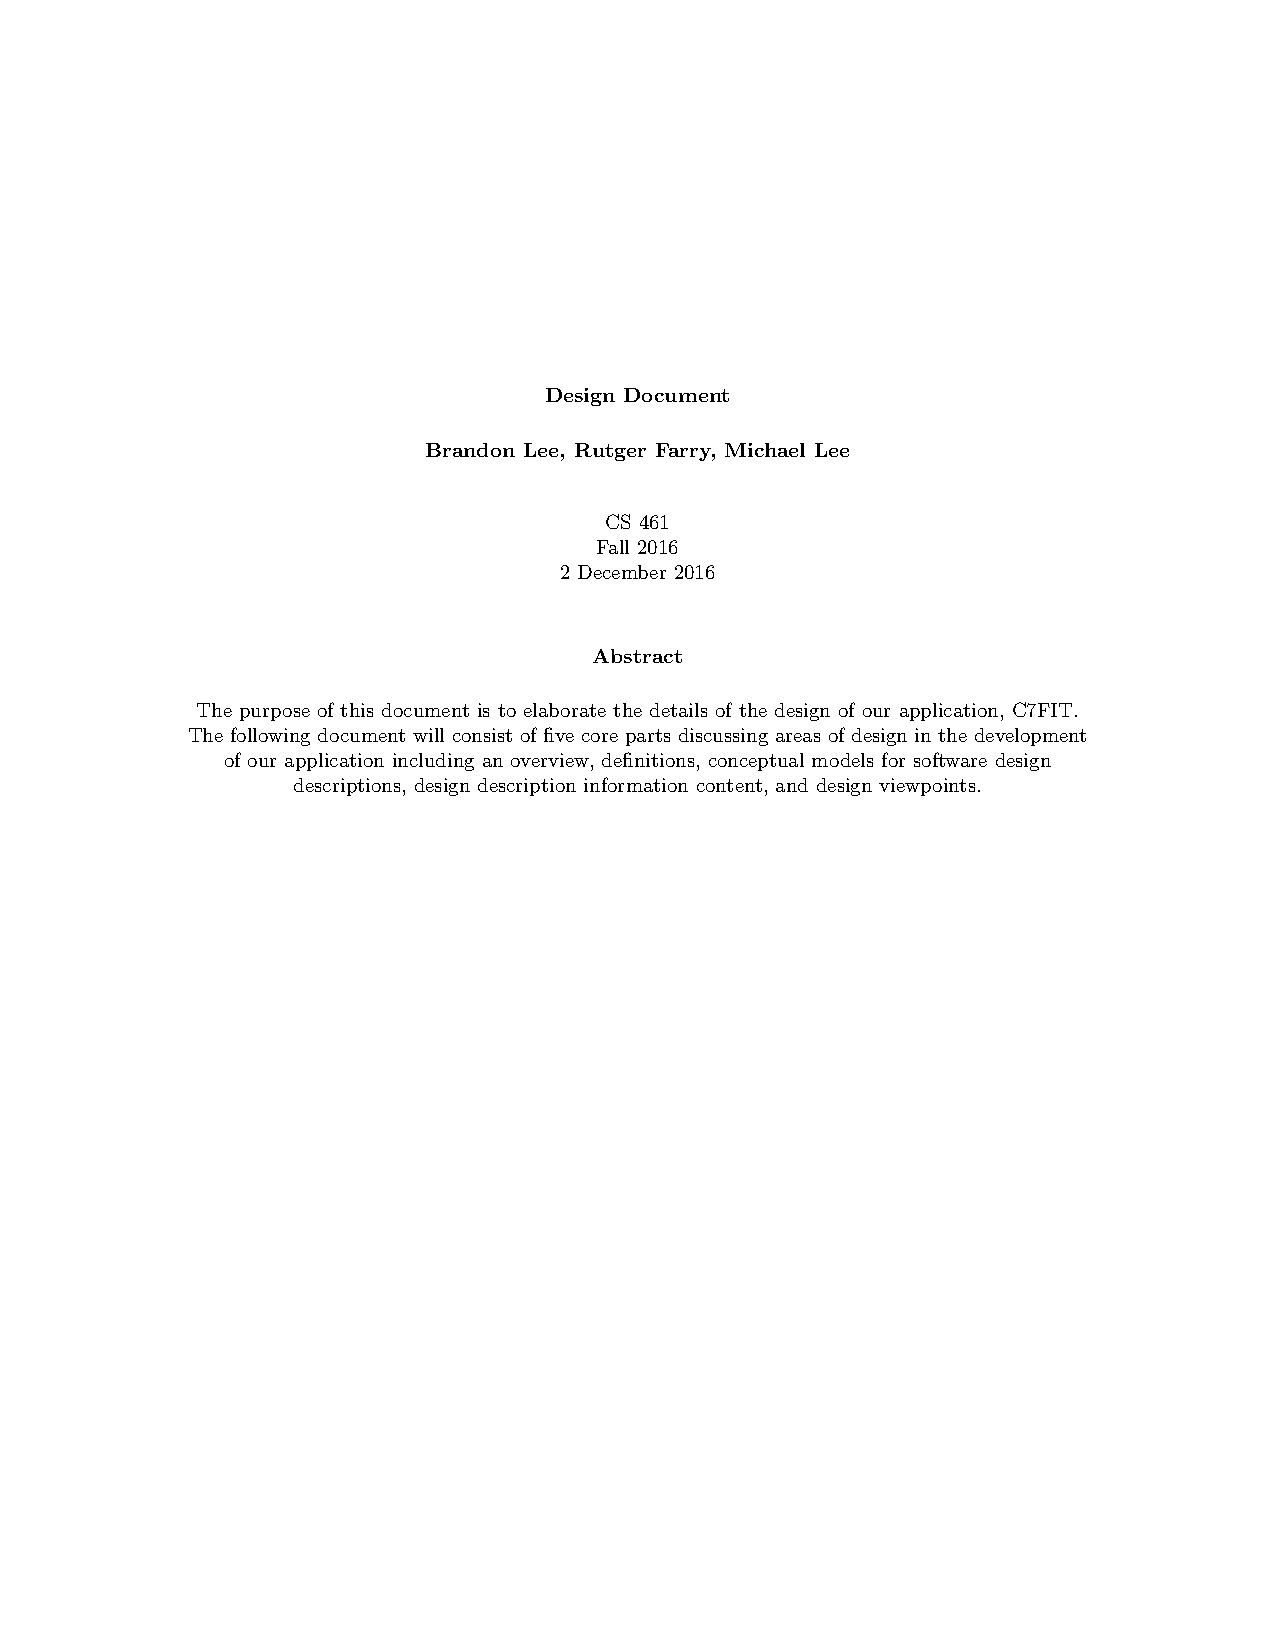
\includepdf[pages={1-},scale=1.0]{pdf/design-doc}
\import{tex/}{design-doc-changes}

% 5
\section{Original Tech Review}
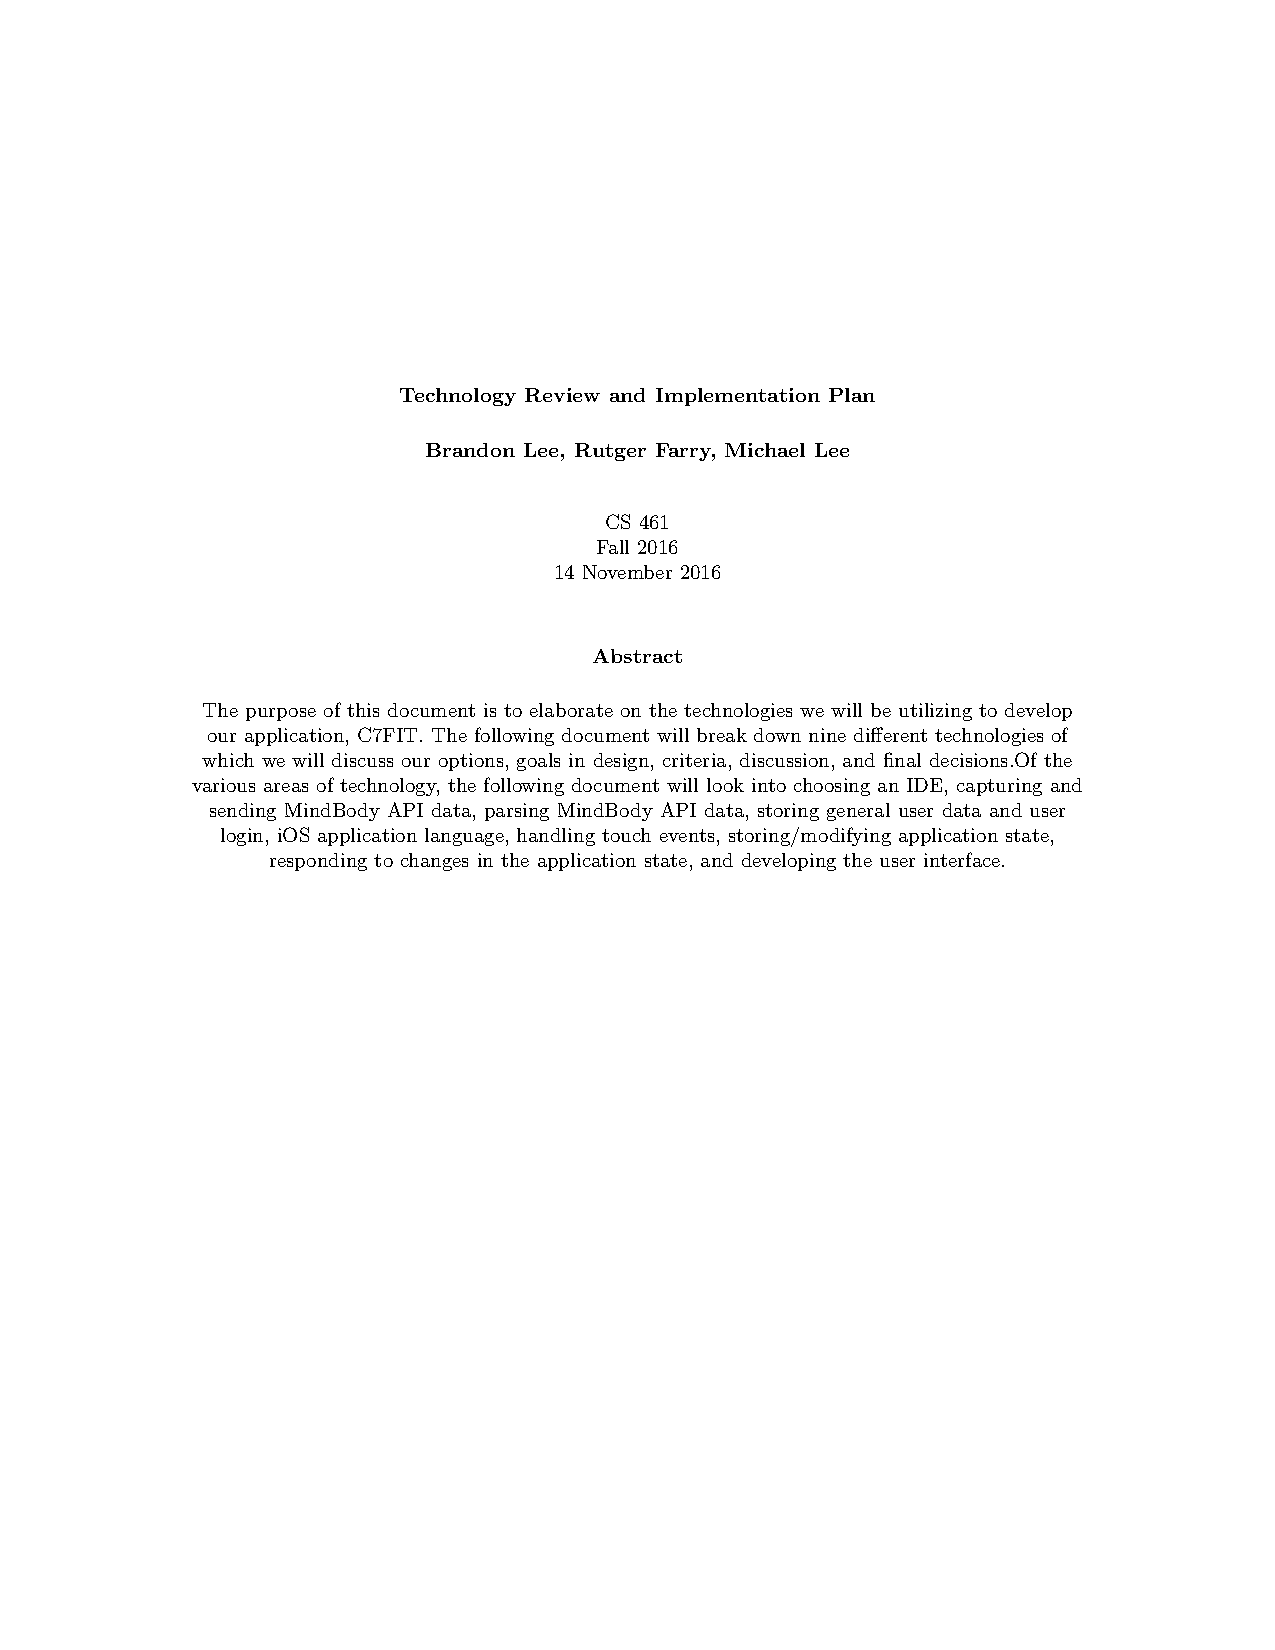
\includepdf[pages={1-},scale=1.0]{pdf/tech-review}
\import{tex/}{tech-doc-changes}

% 6
\section{Weekly Blog Posts}
\import{tex/}{blog-posts-brandon}
\import{tex/}{blog-posts-rutger}
\import{tex/}{blog-posts-michael}

% 7
\section{Final Poster}
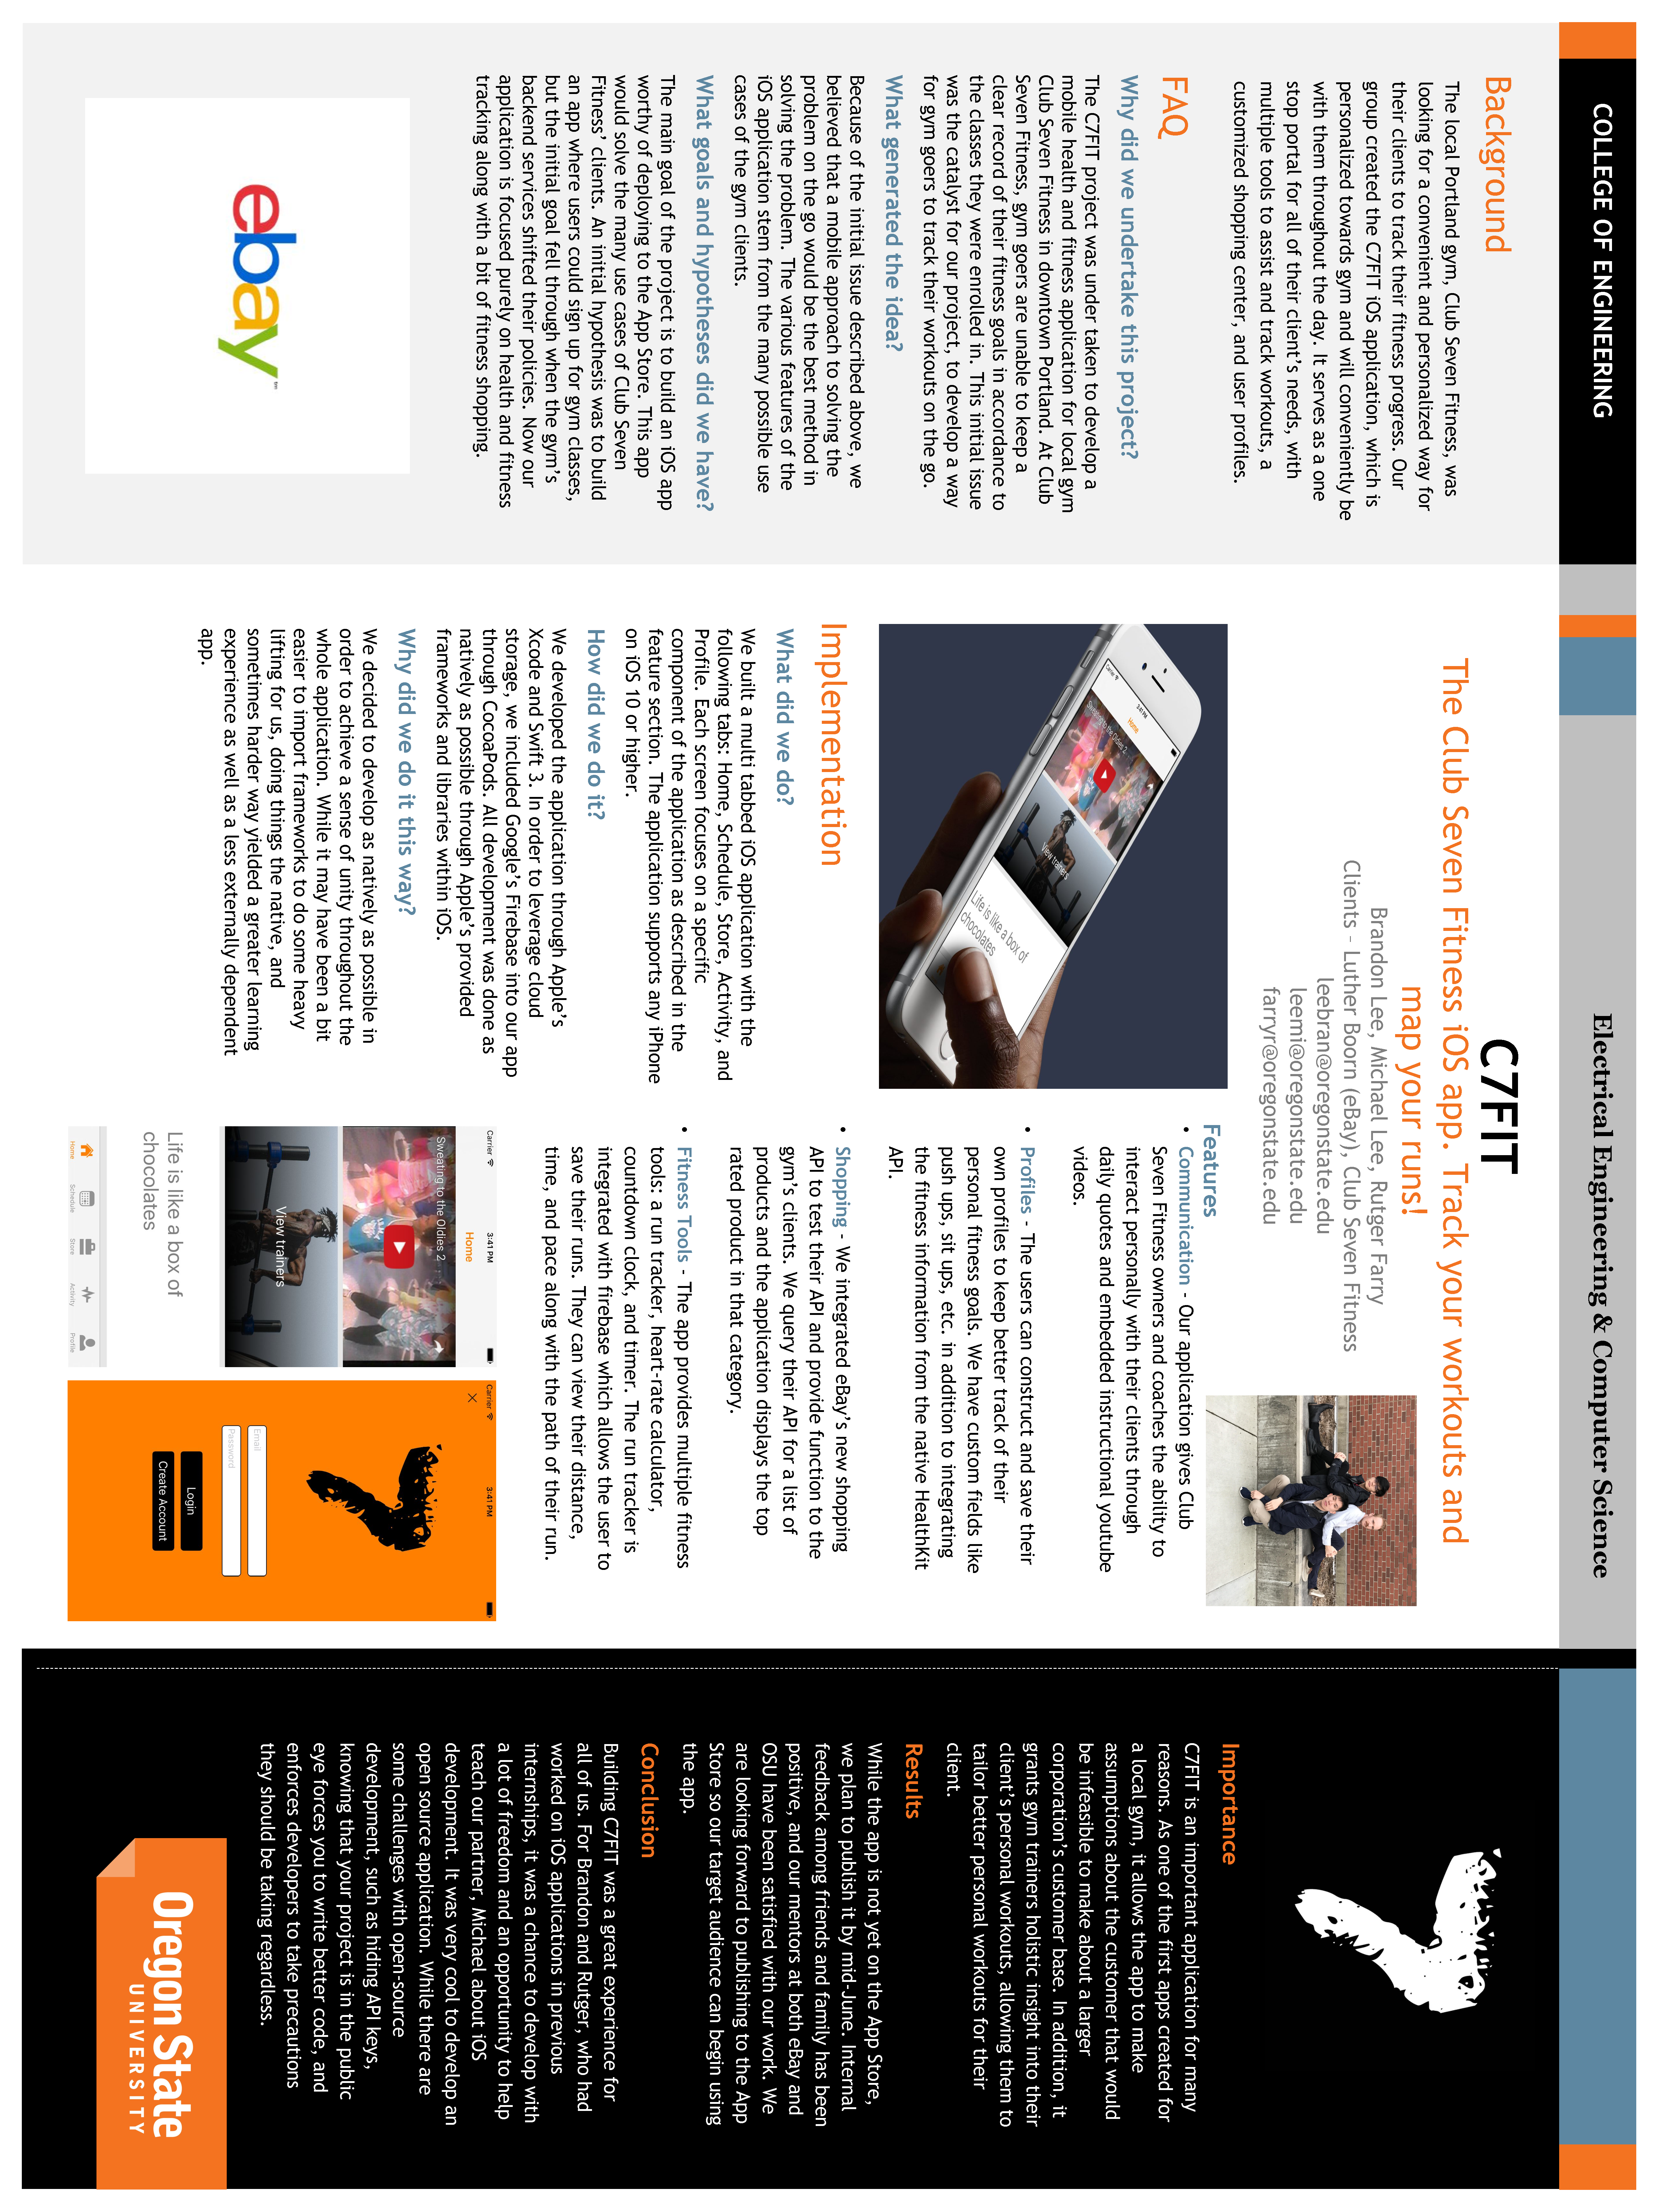
\includepdf[pages={1-},scale=1.0]{pdf/poster}

% 8
\section{Project Documentation}
\import{tex/}{project-documentation}

% 9
\section{Learning New Technologies}
\import{tex/}{learning-new-technologies}

% 10
\section{What We Learned}
\import{tex/}{what-we-learned}

% 11
\section{Appendix I:\ Essential Code}
\import{tex/}{appendix-one}

% 12
\section{Appendix II:\ Pictures and more}
\import{tex/}{appendix-two}

\end{document}
